% CREATED BY DAVID FRISK, 2016
\chapter{Concept Propagation} \label{ch4}
After a set of concepts is known, it can be useful to be able to look for the corresponding concrete expressions in a new language. In this chapter, we describe our approach to this task and present an evaluation of the corresponding module.

\section{Method and implementation}
As mentioned in Section \ref{aligns}, Concept Propagation (CP) is the task of finding the concrete expressions corresponding to a set of known concepts, represented by a set of alignments and/or their abstract representations. Since our method for propagating concepts makes use of dependency tree alignments only, CP can take place before and, in general, independently from a potential conversion of the UD trees into GF trees. \smallskip

There are two scenarios in which CP can prove useful:\smallskip
\begin{enumerate}
    \item when working on a parallel text $A$ in more than two languages. In this case, CP can be used, after CE has been performed on a pair of languages $\langle L_1,L_2 \rangle$, to propagate the extracted alignments in a third version of the text in a new language $L_3$. In this case, the expectation is for the program to be able to propagate the vast majority\footnote{even though handling common translation divergences help, free translation involving radical differences in sentence structure can make it so that some concepts lack a clear counterpart in the text in $L_3$.} of the concepts in the set
    \item when working on two bilingual parallel texts $A$ and $B$ with one language in common, say $A$ in two languages $\langle L_1,L_2 \rangle$ and $B$ in two languages $\langle L_2, L_3 \rangle$. After performing CE on the first pair, CP can be used to look for the extracted concepts in the $L_2$ version of the second and, if they do appear in such text, find their counterparts in $L_3$. Of course, the number of concepts that can be propagated in this scenario can be significantly lower, especially if the two parallel texts do not belong to the same domain.
\end{enumerate}\smallskip

\begin{figure}[h]
    \centering
    \begin{subfigure}{.5\textwidth}
      \centering
      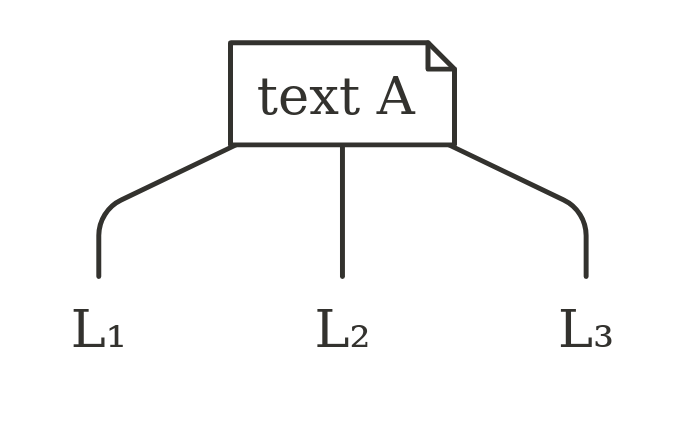
\includegraphics[width=.7\linewidth]{figure/scen1.png}
    \end{subfigure}%
    \begin{subfigure}{.5\textwidth}
        \centering
        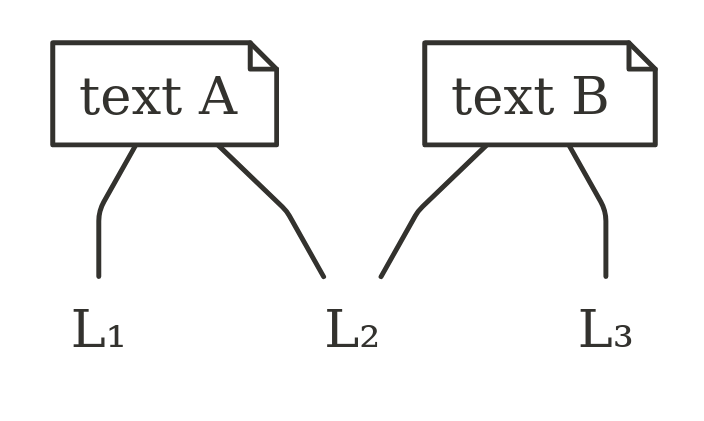
\includegraphics[width=.7\linewidth]{figure/scen2.png}
    \end{subfigure}
    \caption[The two CP scenarios compared]{The two CP scenarios compared. On the left, Scenario 1, when CP is applied on three translations of the same text. On the right, Scenario 2, dealing with two distinct bilingual texts.}
    \label{scens}
\end{figure}

Our algorithm is meant to be as general as possible, and as such it is not optimized for the first scenario, but rather covers both without making any assumptions in terms of sentence alignment\footnote{a way to make the algorithm more efficient for the first scenario could in fact be to rely on the fact that the $n$-lingual parallel text is sentence-aligned, keep track of the sentence from which a particular concept has been extracted and only try to find a equivalent in the corresponding $L_3$ sentence.}. 
It works as follows: for each alignment obtained by performing CE on text $A$, we consider the dependency tree in language $L_2$. We then look for such tree among all subtrees the $L_2$ version of text $B$ is composed of. If a sentence in the $L_2$ version of text $B$ does contain $a_i^2$, we align such sentence to its $L_3$ counterpart using the same procedure as described in Section \ref{extrain} for CE. Finally, if multiple possible correspondences are found, the $L_3$ dependency subtree which is closest in depth to $a_i^2$ is selected. This is meant to avoid, for instance, mistakenly aligning a full sentence tree to a dependency tree extracted when aligning heads, which would otherwise be likely, as their heads are obviously both labelled \texttt{root}. In the next two sections, we discuss some important details of the algorithm, and in Section \ref{heads2} in particular will get to other issues related to head alignment.

\begin{figure}[H]
    \centering
    \lstinputlisting{pseudocode/Propagate.hs}
    \caption[The CP algorithm]{The CP algorithm. The concept to propagate is looked for among the SL subtree of each alignment obtained by comparing the sentences of the new corpus. If it is found, the alignment it belongs to is returned. If there are multiple possible alignments, the alignment whose TL side is closest in depth to the concept itself is returned.}
    \label{prop}
\end{figure}

\subsection{Ignoring details of UD trees}
One point that becomes of extreme importance when dealing with Scenario 2, i.e. when the text used for CP is not a translation of the one used for CE, is the way we look for subtrees in the $L_2$ version of text $B$. Since we work with two different $L_2$ texts, in fact, we cannot expect text $B$'s subtrees to match $L_2$ concepts extracted from $T_1$ exactly: as we saw in Section \ref{ce}, nodes of UD trees contain information, particularly about the position of each word and its head, that should be disregarded in this context.\smallskip 

To make the CP algorithm more robust to minor parse errors, our decision was to consider two (sub)trees equivalent based on a comparison of just their shape and their \texttt{FORM}, \texttt{LEMMA}, \texttt{UPOS} and \texttt{DEPREL} fields. 
In this way, not only all optional fields (which might well differ or be blank for only one of the texts), but word position information is also ignored. 

\subsection{Propagating head alignments} \label{heads2}
The propagation of head alignments is by far the most challenging aspect of CP. 
This is due to the fact that the head of a dependency tree $t$, as defined for the purposes of CE (cf. Section \ref{heads}), is not, strictly speaking, a subtree of $t$ (even though in a broader sense it is, of course, a part of $t$). When head alignments are extracted, in fact, their members are either: \smallskip

\begin{itemize}
    \item trees composed exclusively of the root of a dependency subtree
    \item trees composed of the root of a dependency subtree and some of its immediate subtrees. As discussed in Section \ref{heads}, this happens in cases such as when the root in the SL is a compound (written as a one-word) and its TL counterpart is a multiword.
\end{itemize} \smallskip

Not only, then, is it necessary to look for each concept to propagate among all the dependency subtrees of each SL sentence of the corpus CP is performed on, but for each subtree it is also necessary to check whether the concept could be a head of such subtree. This is implemented by means of a function \texttt{isHeadOf} specular to \texttt{alignHeads}. \smallskip

If this is the case, i.e. if the concept the program is trying to propagate is the head of a certain SL subtree, then the resulting alignment should be with the head of the TL counterpart of such subtree.

\section{Evaluation} \label{eval3}
In the following three sections, we describe both the CP experiments performed and their results. Clearly, for all the experiments, we make use of the evaluation script used for CE, which has been extended to also compute CP-specific statistics, such as the percentage of (successfully) propagated concepts.

\subsection{Preliminary testing} 
One way to check the CP module for obvious flaws before trying to assess its performance in the two scenarios described above is to try to re-obtain the alignments obtained with the CE module via propagation. This means running both programs on the exact same input treebanks as used for CE. It represents a special case of Scenario 1 in which the program is expected to be able to propagate all alignments, with no exceptions. \smallskip 

The fact that many of the alignments obtained via propagation are the same as the ones extracted initially is generally a good indication that the program is working according to expectations. However, this has to be taken with a grain of salt: as discussed in the above, the program looks for one possible counterpart per concept only and is provided no indication about what sentence in particular it should look into, so that in presence of multiple valid alternative alignments the user should not expect it to identify the same correspondences as the extraction procedure, but rather just correct, potentially different correspondences. 

\subsubsection{Experimental results} \label{eval4r}
This kind of pre-evaluation has been run on the first 100 sentences of the PUD treebanks in English and Italian, one of the corpora used for evaluating CE. Most importantly, the experiment confirms that the CP module is in fact able to find all the alignments extracted by CE. 
The results also show that the vast majority of the propagated alignments is identical to its extracted counterpart, and that most often, even when it is not, that does not imply that the propagated alignment is incorrect. Out of a total of 224 (18.69\%) incorrect propagated alignments, only 28 (12.5\%) introduce an alignment error which was not already present in their extracted counterparts, and there are even instances where propagated alignments are, conincidentally, correct even though their extracted counterparts are not.

\subsection{Scenario 1}
For evaluating how well CP works in the first scenario, the corpus we use is the same as for testing, but in three instead of two languages: the concept extracted by means of comparing the English to the Italian version are propagated to Swedish, using both English and Italian UD trees as the starting point. \smallskip

Considering that we are working with three versions of the same text, the expectation is for the program to be able to propagate the vast majority of the concepts with a precision similar to that obtained during the extraction stage, even though free translation, unhandled translation divergences and annotation inconsistencies can make it possible for some of them not to be found in the Swedish translation or not to be aligned correctly. \smallskip

As for when it comes for CE, comparing the results of CP for two different language pairs, English-Swedish and Italian-Swedish, can be interesting to see how much easier it is to propagate concepts in two more syntactically similar languages.

\subsubsection{Experimental results}
As Table \ref{tcp1} shows, the experimental results of this type of evaluation match the above expectations. First, the number of alignments the program is able to propagate is, for both language pairs, smaller than that obtained in the testing phase but still relatively large, while the amount of propagation errors increases marginally. Furthermore, the English-Swedish pair gives slightly better results than the Italian-Swedish pair, both in terms of the number of alignments the program is able to propagate and in terms of the amount of alignment errors. \smallskip

It is interesting to notice, however, that the amount of errors is significantly (> 5\%) inferior when concepts are propagated to Swedish starting from English, as opposed to Italian, dependency trees. This is most likely due to the syntactical features shared by the former two languages. This means that not all Italian-English extraction errors are propagated and it seems to suggest that, if we were to only use the trilingual alignments obtained by English-Italian extraction followed by English-Swedish propagation, some of the initial incorrectly extracted alignments would be automatically discarded.

\begin{table}[H]
    \centering
    \begin{tabular}{|l|l|l|}
    \hline
    \textbf{}              & \textbf{en-sv} & \textbf{it-sv} \\ \hline
    propagated             & 1019 (85.05\%) & 979 (84.64\%) \\ \hline
    tot. errors            & 133 (13.05\%)  & 187 (19.1\%)  \\ \hline
    CP-introduced          & 75 (56.39\%)   & 84 (44.91\%)   \\ \hline
    \end{tabular}
    \caption[Performance of CP Scenario 1 on manually annotated data]{Results of propagating the Italian-English alignments obtained via CE on the first 100 sentences of the PUD corpus to Swedish, using either the English or Italian subtrees as a starting point.}
    \label{tcp1}
    \end{table}

\subsection{Scenario 2}

The PUD corpus is composed of extracts of texts on a variety of subjects. As a consequence, performing an evaluation of CP in Scenario 2 using, for extraction and propagation, two different subsets of the corpus, would not help assess whether the module is well suited for the most relevant subcase of such scenario, i.e. when working with two texts belonging to the same domain. \smallskip

On top of evaluating the program on PUD data dividing the set of sentences used so far into two equally sized subsets, then, the two course plans corpora described in Section \ref{plans} have been also used to put the program to the test. \smallskip

These two small bilingual corpora allow us to perform two additional experiments: \smallskip
\begin{enumerate}
    \item to extract English-Swedish alignments from the CSE corpus and propagate them to Italian using the DMI corpus
    \item vice versa, to extract English-Italian alignments from the DMI corpus and propagate them to Swedish using the CSE corpus
\end{enumerate} \smallskip

\subsubsection{Experimental results}

\paragraph{Propagation with texts in different domains}
When it comes to the first set of experiments, where we use PUD data, being the subsets of selected sentences extremely small and having the correctness of most alignments been already assessed in previous experiments, it is easy to work with all possible pairs of languages. The results, summarized in Table \ref{tcp2pud}, show that, in general, only a small fraction of the extracted alignments are actually propagated in this case. As mentioned above, this is to be expected since different sentences belong to different domain. A closer look to the set of alignments returned by propagation, the vast majority of which has single words as members, shows that most of them are common function words, which, alone, are not always relevant for a GF-based MT pipeline. 
Common determiners such as articles, for instance, can be better handled by RGL grammars alone. 
Prepositions, on the other hand, are only useful with some information about the context in which they occur in, since it is customary for them to be used differently across different, even closely related languages. 
However, some common content words, like $\langle$\textit{always, sempre, alltid}$\rangle$, $\langle$\textit{new, nuovi, nya}$\rangle$ and $\langle$\textit{same, stesso, samma}$\rangle$ are also aligned correctly.

\begin{table}[H]
    \centering
    \scriptsize
    \begin{tabular}{|l|l|l|l|l|l|l|}
    \hline
    \textbf{}                     & \textbf{en-it-sv} & \textbf{it-en-sv} & \textbf{en-sv-it} & \textbf{sv-en-it} & \textbf{it-sv-en} & \textbf{sv-it-en} \\ \hline
    extracted   & 638               & 638               & 687               & 687               & 608               & 608               \\ \hline
    propagated                    & 92 (14.42\%)      & 92 (14.42\%)      & 98 (14.26\%)      & 84 (12.22\%)      & 101 (16.61\%)     & 87 (14.37\%)      \\ \hline
    tot. errors                   & 46 (50\%)         & 21 (22.82\%)      & 42 (42.85\%)      & 24 (28.57\%)      & 21 (20.79\%)      & 28 (32.18\%)      \\ \hline
    CP-introduced                 & 33 (71.73\%)      & 11 (52.38\%)      & 21 (50\%)         & 12 (50\%)         & 12 (57.14\%)      & 21 (75\%)         \\ \hline
    \end{tabular}
    \caption[Performance of CP Scenario 2 on manually annotated non-homogeneous data]{Results of CP for various language pairs using PUD (non-homogeneous) data. For each column, the first two languages are the ones used for extraction and the second two the ones used for propagation.}
    \label{tcp2pud}
    \end{table}

The table also shows, like the results obtained from Scenario 1 suggest too, that the order in which languages are used is not completely irrelevant: while the percentage of propagated alignments does not vary widely, the amount of errors is significantly lower when the propagation step involves the two syntactically more similar languages, English and Swedish. The fact that CP works better with English-Italian than with Italian-Swedish, on the other hand, may simply be a result of the fact that the latter language pair was never used for testing the program during its development, which might have caused some of the criteria to be not completely language pair-independent. \smallskip

Finally, the percentage of errors introduced by CP is significantly higher than that recorded for Scenario 1. One factor that contributes to this is the fact that function words, which are by far more numerous in the propagated alignments than content words, are often used differently in different languages and contexts. When it comes to the languages we are considering, this applies in particular to prepositions: because it is hard to know what the correct translation equivalent is without looking at the specific sentence, when CP is performed on a text different from the one used for CE, many preposition-to-preposition alignments have to be marked as incorrect even though they might be correct in some specific cases.

\paragraph{Propagation with texts within the same domains}

Quantitatively, the results of the last pair of experiments, performed on two different automatically parsed bilingual corpora composed of course plans of Computer Science programmes, are to some extent similar to those obtained using different texts in different domains (cf. Tables \ref{tcp2courses} and \ref{tcp2pud}). Only a tiny fraction of the extracted alignments is propagated and errors are numerous, as in the previous setting. 

\begin{table}[H]
    \centering
    \begin{tabular}{|l|l|l|}
    \hline
                           & \textbf{sv-en-it} & \textbf{it-en-sv} \\ \hline
    extracted concepts     & 1950              & 1823              \\ \hline
    propagated             & 205 (10.51\%)     & 200 (10.97\%)     \\ \hline
    tot. errors            & 66 (32.19\%)      & 61 (30.5\%)       \\ \hline
    errors introduced by CP & 33 (50\%)        & 33 (54.09\%)      \\ \hline
    \end{tabular}
    \caption[Performance of CP Scenario 2 on automatically parsed homogeneous data]{Results of CP for using two different bilingual corpora belonging to the same domain of course plans. For each column, the first two languages are the ones used for extraction and the second two the ones used for propagation.}
    \label{tcp2courses}
    \end{table}

    More than the quantitative results, however, it is interesting to take a look at some of the propagated concepts. Because the text are similar both stylistically and, most importantly, in terms of content, the program is in this case also able to find trilingual correspondences between content words, sometimed specific of the domain. Examples of such alignments are $\langle$\textit{skills, capacità, färdigheter}$\rangle$, $\langle$\textit{functional, funzionale, funktionell}$\rangle$, $\langle$\textit{exam, prova, tentamen}$\rangle$, $\langle$\textit{course, corso, kurs}$\rangle$, $\langle$\textit{prerequisites, prerequisiti, behörigheter}$\rangle$, $\langle$\textit{lectures, lezioni, föreläsningar}$\rangle$ and $\langle$\textit{knowledge, conoscenza, kunskap}$\rangle$. \smallskip

    Sometimes, however, the meaning of a word is highly context-dependent and as a consequence, even if both the pairs of extracted and propagated alignments are correct, the corresponding trilingual alignment we could infer isn't (e.g. $\langle$\textit{learning, conoscere}$\rangle$ and $\langle$\textit{learning, inlärning}$\rangle$). \smallskip

    Finally, in some rare cases, even correspondences regarding longer expressions, such as $\langle$\textit{the aim of the course, l'obiettivo del corso, syftet med kursen}$\rangle$, can be found. In this case, the English-Italian correspondence is not especially useful, since the phrase could be translated almost word by word between the two languages, but the translation to Swedish is not literal, thus making the alignment useful for the purposes of MT.